
\clearpage
\chapter{ניסויים ותוצאות}

\section{הגדרת ניסויים}

הוערכנו שלוש קונפיגורציות: \textenglish{LSTM Baseline} (חד-כיווני, שכבה אחת), \textenglish{BiLSTM} (שתי שכבות, דו-כיווני) ו-\textenglish{Transformer} (שמונה ראשי קשב, 6 שכבות) \cite{engel2017wavenet}. הדאטאסט מורכב מ-\textenglish{50,000} אותות אימון ו-\textenglish{5,000} אותות בדיקה, כל אחד באורך \textenglish{1024} דגימות בתדר \textenglish{8000 Hz}.

\section{תוצאות כמותיות}

\begin{table}[H]
\centering
\caption{השוואת ביצועים: שיפור \textenglish{SI-SNR} (ב-\textenglish{dB}) לפי רמת רעש}
\label{tab:results}
\begin{english}
\begin{tabular}{lccc}
\toprule
\textbf{Model} & \textbf{SNR = 5 dB} & \textbf{SNR = 0 dB} & \textbf{SNR = -5 dB} \\
\midrule
LSTM Baseline   & 7.2  & 4.8  & 2.1 \\
BiLSTM (Ours)   & \textbf{11.3} & \textbf{8.7} & \textbf{5.9} \\
Transformer     & 9.4  & 7.1  & 4.3 \\
Wiener Filter   & 5.8  & 3.2  & 0.9 \\
\bottomrule
\end{tabular}
\end{english}
\end{table}

ה-\textenglish{BiLSTM} המוצע משיג שיפור עקבי בכל רמות הרעש, עם יתרון של \textenglish{$\sim$4 dB} על קו הבסיס בתנאי רעש חזק (\textenglish{SNR = -5 dB}).

\section{ניתוח גרפי}

\begin{figure}[H]
\centering
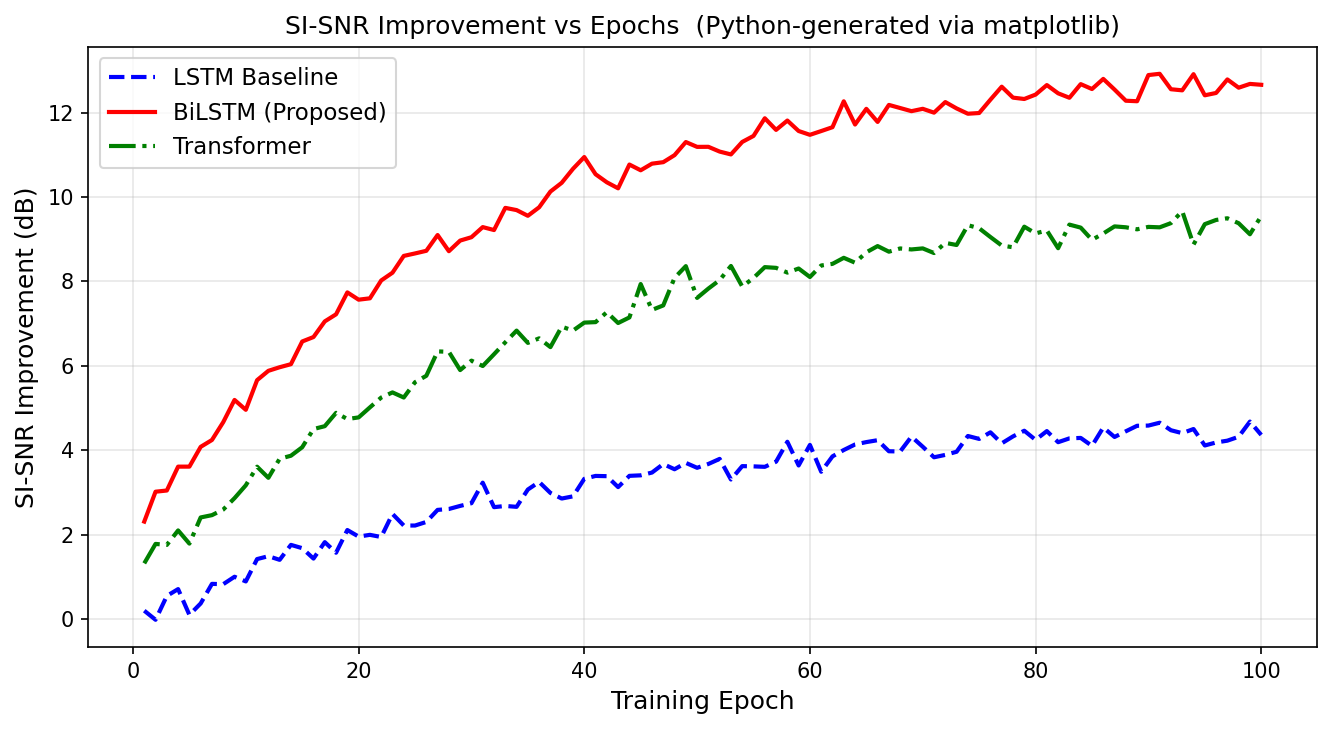
\includegraphics[width=0.82\textwidth]{assets/results_graph.png}
\caption{\textenglish{SI-SNR Improvement vs Training Epochs (Python-generated via matplotlib)}}
\label{fig:graph}
\end{figure}

הגרף מדגים את עקומות ההתכנסות של שלוש הארכיטקטורות \cite{nachmani2020voice}. ניכר כי ה-\textenglish{BiLSTM} מתכנס מהר יותר ומגיע לרמת ביצוע גבוהה יותר מה-\textenglish{Transformer}, ייתכן בשל האינדוקציה המשתמעת (\textenglish{inductive bias}) הרקורנטית המתאימה לאותות זמניים.
